\RequirePackage{fix-cm}
\documentclass[12pt]{article}
% fonts

\usepackage[T1]{fontenc}
\usepackage{newtxtext}
\usepackage{microtype}
\usepackage{bm}
\usepackage{amsthm} % before newtxmath b/c latex
\usepackage{newtxmath}
\usepackage[bb=ams,cal=cm]{mathalpha} % mt variants need MathTime Pro (not installed); matches template/preamble.tex

\usepackage{amsmath}
\usepackage{amsfonts}
\usepackage{thmtools}
\usepackage{mathtools}

% figures and tables

\usepackage{graphicx}
\usepackage{booktabs}

% spacing

\usepackage[parfill]{parskip}
\setlength{\parindent}{0pt}
\setlength{\parskip}{2ex plus 0.2ex minus 0.2ex}

% geometry of the page

\usepackage[
paper  = letterpaper,
left   = 1in,
right  = 1in,
top    = 1in,
bottom = 1in,
]{geometry}

% references

\usepackage[round]{natbib}
\usepackage[hidelinks]{hyperref}

\usepackage{tikz}
\usetikzlibrary{positioning,fit,arrows.meta}
% Generated by q1_cavi.py; do not edit numerical values manually.
\newcommand{\qoneUsers}{80}
\newcommand{\qoneItems}{60}
\newcommand{\qoneK}{3}
\newcommand{\qoneNoise}{0.5}
\newcommand{\qoneTrain}{1874}
\newcommand{\qoneTest}{2926}
\newcommand{\qoneRMSE}{0.559}
\newcommand{\qoneBaseline}{1.751}
\newcommand{\qoneOracle}{0.495}
\newcommand{\qoneCoverage}{94.4}
\newcommand{\qoneSeed}{20261111}

% Generated by q2_kl.py; do not edit.
\newcommand{\klSeed}{20261111}
\newcommand{\klGridN}{2916}
\newcommand{\klBestM}{3.0}
\newcommand{\klBestSigma}{1.0}
\newcommand{\klBestMC}{0.68930}
\newcommand{\klBestSE}{0.00074}
\newcommand{\klBestQuad}{0.68930}
\newcommand{\klForwardSigma}{3.16228}
\newcommand{\klReverseAtForward}{0.9380}

% Generated by check_kl.py.
\newcommand{\klContinuousAbsM}{2.984}
\newcommand{\klContinuousSigma}{1.023}
\newcommand{\klContinuousD}{0.68877}

% Generated by check_preferences.py.
\newcommand{\prefLinearPct}{99.8}
\newcommand{\prefWidePct}{84.5}
\newcommand{\prefNarrowPct}{96.0}
\newcommand{\prefDiagnosticTruth}{0.27}
\newcommand{\prefDiagnosticAtOne}{0.73}
\newcommand{\prefDiagnosticPosterior}{0.72}
\newcommand{\prefTrueRegret}{1}


% Keep the previous homework's fonts, 12pt text, and one-inch margins.
\setlength{\parskip}{0.65ex plus 0.1ex minus 0.1ex}
\setlength{\abovedisplayskip}{4pt plus 1pt minus 1pt}
\setlength{\belowdisplayskip}{4pt plus 1pt minus 1pt}
\setlength{\abovedisplayshortskip}{3pt}
\setlength{\belowdisplayshortskip}{3pt}
\newcommand{\E}{\mathbb{E}}
\newcommand{\Var}{\operatorname{Var}}
\newcommand{\tr}{\operatorname{tr}}
\newcommand{\KL}{\operatorname{KL}}
\newcommand{\N}{\mathcal{N}}

\begin{document}
\begin{flushleft}
\textbf{Homework 2}\\
Jaisel Singh (js6897) \hfill November 13, 2026
\end{flushleft}

\textbf{Question 1: Variational Inference for Matrix Factorization}

\textit{(a) Coordinate updates.}
Write $\Omega_i=\{j:(i,j)\in\Omega\}$, $\Omega^j=\{i:(i,j)\in\Omega\}$,
and let $(\mu_i,S_i)$ and $(\nu_j,T_j)$ be the means and covariances of the
user and item factors. CAVI sets $\log q^*(u_i)=\E_{q_{-u_i}}[\log p(r_\Omega,U,V)]+C$:
\[
\begin{aligned}
\log q^*(u_i)
&=-\tfrac12u_i^\top u_i
  -\frac{1}{2\sigma^2}\sum\nolimits_{j\in\Omega_i}\E_{q(v_j)}[(r_{ij}-u_i^\top v_j)^2]+C\\
&=-\tfrac12u_i^\top\!\bigl[I_K+\sigma^{-2}\sum\nolimits_{j\in\Omega_i}\E_q[v_jv_j^\top]\bigr]u_i
  +\sigma^{-2}u_i^\top\sum\nolimits_{j\in\Omega_i}r_{ij}\nu_j+C.
\end{aligned}
\]
Here $C$ is constant in $u_i$. Completing the square gives $q^*(u_i)=\N(\mu_i,S_i)$, with
\[
\boxed{\quad
S_i=\bigl[I_K+\sigma^{-2}\sum\nolimits_{j\in\Omega_i}\E_q[v_jv_j^\top]\bigr]^{-1},\quad
\mu_i=\sigma^{-2}S_i\sum\nolimits_{j\in\Omega_i}r_{ij}\E_q[v_j].\quad}
\]
Here $\E_q[v_j]=\nu_j$ and $\E_q[v_jv_j^\top]=T_j+\nu_j\nu_j^\top$, so item uncertainty
$T_j$ enters. Each precision is $I_K$ plus positive-semidefinite terms, hence positive
definite. Analogously, $q^*(v_j)=\N(\nu_j,T_j)$ with
\[
T_j=\bigl[I_K+\sigma^{-2}\sum\nolimits_{i\in\Omega^j}(S_i+\mu_i\mu_i^\top)\bigr]^{-1},\qquad
\nu_j=\sigma^{-2}T_j\sum\nolimits_{i\in\Omega^j}r_{ij}\mu_i.
\]

\textit{(b) Graphical model.}
\begin{center}
\begin{minipage}{0.49\linewidth}
\centering
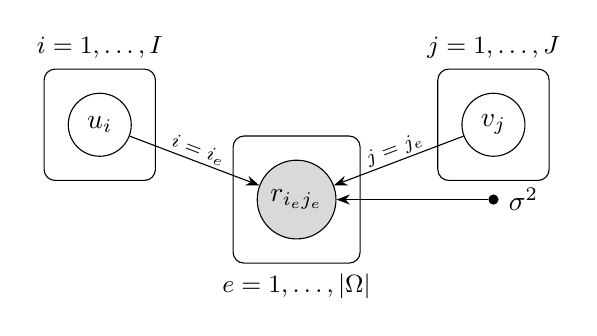
\begin{tikzpicture}[>=Stealth,
 latent/.style={circle,draw,minimum size=8mm,inner sep=1pt},
 observed/.style={circle,draw,fill=black!15,minimum size=10mm,inner sep=1pt},
 plate/.style={draw,rounded corners,inner sep=3mm}]
 \node[latent] (u) at (0,0) {$u_i$};
 \node[latent] (v) at (5.0,0) {$v_j$};
 \node[observed] (r) at (2.5,-0.95) {$r_{i_ej_e}$};
 \node[plate,fit=(u),label={[font=\small]above:$i=1,\ldots,I$}] {};
 \node[plate,fit=(v),label={[font=\small]above:$j=1,\ldots,J$}] {};
 \node[plate,fit=(r),label={[font=\small]below:$e=1,\ldots,|\Omega|$}] {};
 \node[circle,fill,inner sep=1.3pt,label=right:$\sigma^2$] (s) at (5.0,-0.95) {};
 \draw[->] (u) -- node[midway,above,sloped,font=\scriptsize,inner sep=1pt] {$i=i_e$} (r);
 \draw[->] (v) -- node[midway,above,sloped,font=\scriptsize,inner sep=1pt] {$j=j_e$} (r);
 \draw[->] (s) -- (r);
\end{tikzpicture}
\end{minipage}\hfill
\begin{minipage}{0.49\linewidth}
Let $\Omega=\{(i_e,j_e)\}_{e=1}^{|\Omega|}$. Shading denotes observed ratings;
arrows select the \emph{shared} user/item nodes indexed by each entry, not fresh
latent vectors per rating. $K$ and $\sigma^2$ are fixed.
\end{minipage}
\end{center}

\textit{(c) Predictive uncertainty.}
For $(i,j)\notin\Omega$, integrate the observation model against $q(u_i)q(v_j)$.
Independence under $q$ and $\E[(u_i^\top v_j)^2]=\tr[(S_i+\mu_i\mu_i^\top)(T_j+\nu_j\nu_j^\top)]$ give
\[
\E_q[r_{ij}]=\mu_i^\top\nu_j,\qquad
\Var_q(r_{ij})=\sigma^2+\tr(S_iT_j)+\mu_i^\top T_j\mu_i+\nu_j^\top S_i\nu_j.
\]
The predictive distribution is generally non-Gaussian. The shared noise $\sigma^2$
adds the same variance to every pair. With no ratings for user $i$, $q(u_i)$ stays at
its prior and $S_i=I_K$; item cold starts are analogous. Draw $u_i,v_j$ from $q$ and
$r_{ij}\sim\N(u_i^\top v_j,\sigma^2)$. Flag pairs whose 95\% predictive interval
exceeds a width chosen for the rating scale. Check interval coverage on held-out
ratings, since mean-field intervals can be too narrow.

\textit{(d) Optional implementation.}
\textnormal{q1\_cavi.py} simulates an $\qoneUsers\times\qoneItems$ matrix with
$K=\qoneK$, $\sigma=\qoneNoise$ and $\qoneTrain$ training ratings; the best of three
random starts is selected by training ELBO. On $\qoneTest$ held-out ratings, RMSE is
$\qoneRMSE$, against $\qoneBaseline$ for zero prediction. The known true mean
$u_i^\top v_j$ yields $\qoneOracle$ on this test set (population noise floor $\sigma=\qoneNoise$). Nominal 95\% interval coverage is
$\qoneCoverage\%$ in this simulation. Every sweep increased the ELBO.

\clearpage
\textbf{Question 2: Understanding Kullback--Leibler Divergence}

\textit{(a) Forward KL: analytic minimizer.}
The target is $p(z)=\tfrac12\N(z;-a,s^2)+\tfrac12\N(z;a,s^2)$ and the approximation
is $q(z)=\N(z;m,\sigma^2)$. The mixture is symmetric, so
\[
\E_p[Z]=0,\qquad
\Var_p(Z)=\E[\Var(Z\mid\text{component})]
  +\Var(\E[Z\mid\text{component}])=s^2+a^2.
\]
Let $V=a^2+s^2$. The entropy $H(p)=-\int p\log p$ does not depend on $(m,\sigma)$;
using $\E_p[(Z-m)^2]=V+m^2$,
\[
\begin{aligned}
\KL(p\|q)
&=-H(p)-\E_p[\log q(Z)]\\
&=-H(p)+\tfrac12\log(2\pi)+\log\sigma+\frac{V+m^2}{2\sigma^2}.
\end{aligned}
\]
For every fixed $\sigma>0$, this is uniquely minimized by $m=0$. Setting
$t=\sigma^2>0$, the remaining derivative is
\[
\frac{d}{dt}\left(\tfrac12\log t+\frac{V}{2t}\right)
=\frac{t-V}{2t^2},
\]
which is negative below $V$ and positive above it. Therefore the unique global fit is
\[
\boxed{\ m_{\rm F}=0,\quad \sigma_{\rm F}=\sqrt{a^2+s^2}.\ }
\qquad (a,s)=(3,1):\quad q_{\rm F}=\N(0,10).
\]

\textit{(b) Reverse KL: the requested Monte Carlo grid search.}
At each of the $81\times36=\klGridN$ points
$m=-4,-3.9,\ldots,4$ and $\sigma=0.5,0.6,\ldots,4$, draw fresh independent
$\epsilon_b\sim\N(0,1)$, set $z_b=m+\sigma\epsilon_b$, and compute
\[
\widehat D(m,\sigma)=\frac{1}{10{,}000}\sum_{b=1}^{10{,}000}
\left[-\log\sigma-\tfrac12\log(2\pi)-\tfrac12\epsilon_b^2-\log p(z_b)\right].
\]
The mixture log density is evaluated by log-sum-exp to avoid underflow.
With NumPy's PCG64 generator, seed $\klSeed$, and $m$ increasing in the outer loop,
the selected grid point is
\[
\boxed{\ (\widehat m_{\rm R},\widehat\sigma_{\rm R})=(\klBestM,\klBestSigma),
\qquad \widehat D=\klBestMC\ \text{nats}.\ }
\]
\begin{center}
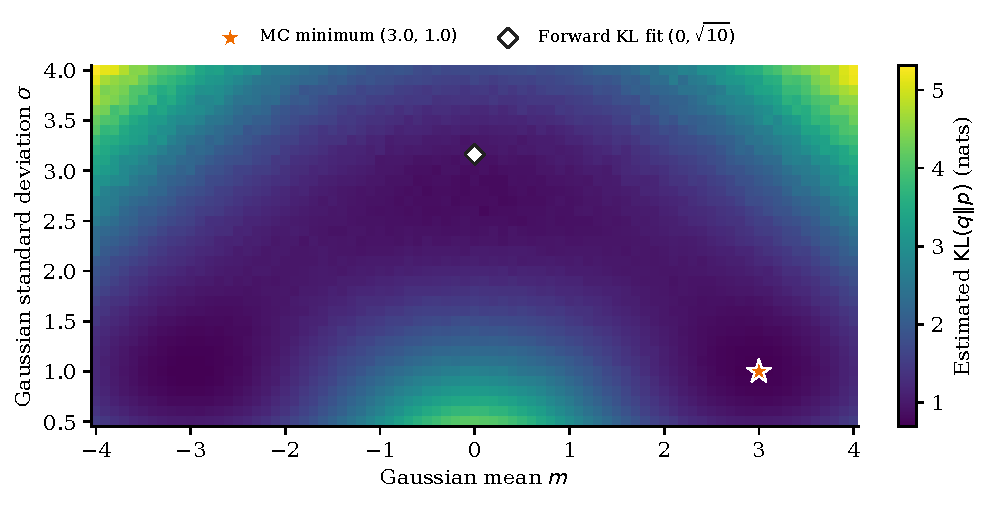
\includegraphics[width=0.83\linewidth]{figures/q2_heatmap.pdf}
\end{center}
{\small Figure 1. The estimated reverse KL on the full prescribed grid;
the star marks its minimum. The diamond is the forward-KL fit.}

\clearpage
\textbf{Question 2 (continued): approximation and interpretation}

\textit{(c) Compare the densities.}
\begin{center}
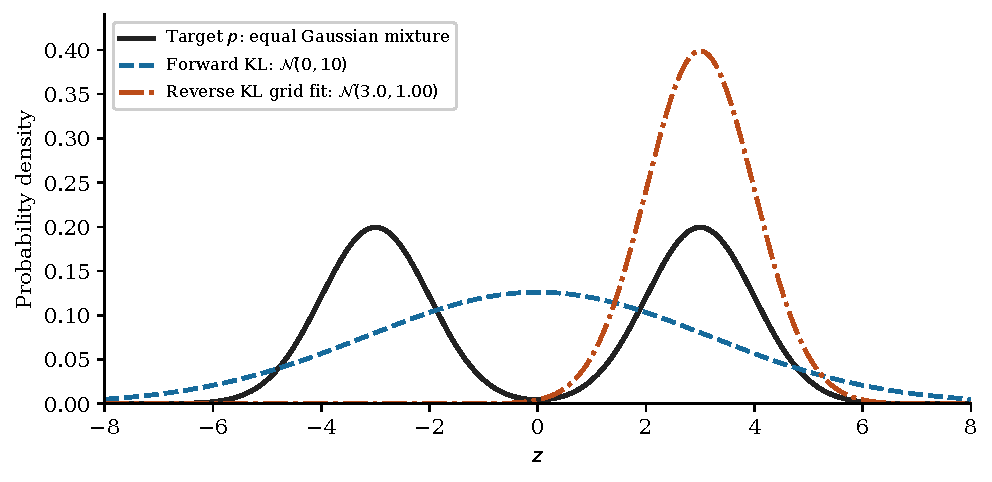
\includegraphics[width=0.94\linewidth]{figures/q2_densities.pdf}
\end{center}
{\small Figure 2. The target mixture, the analytic forward-KL Gaussian,
and the Gaussian selected by the Monte Carlo reverse-KL grid search.}

\textbf{Why forward KL covers modes.}
In $\KL(p\|q)=\E_p[\log p(Z)-\log q(Z)]$, the expectation samples both modes
of $p$. A $q$ that assigns little density near either mode incurs a large
cross-entropy cost there. Within the single-Gaussian family, the best solution
matches the target's mean and variance: its mean lies between the modes and its
standard deviation is $\sqrt{10}\approx\klForwardSigma$.
It covers both modes but also places substantial mass in the valley between
them. Matching two moments cannot reproduce bimodality.

\textbf{Why reverse KL seeks a mode here.}
In $\KL(q\|p)=\E_q[\log q(Z)-\log p(Z)]$, the expectation instead samples
where $q$ puts mass. A broad Gaussian pays for placing samples in the low-density
valley of $p$. Concentrating near one component largely avoids that valley;
the other mode contributes little because $q$ rarely samples it. The selected
$\N(3,1)$ therefore approximates one component rather than the entire mixture.
Indeed, near $z=3$, $p(z)\approx\tfrac12\N(z;3,1)$, so
$\log(q(z)/p(z))\approx\log 2$, consistent with the computed value just below
$\log 2\approx0.69315$. The small overlap of the components makes the value
slightly smaller.

\textbf{Symmetry and numerical accuracy.}
Because $p(-z)=p(z)$, a change of variable $z\mapsto-z$ gives
\[
\KL(\N(m,\sigma^2)\|p)=\KL(\N(-m,\sigma^2)\|p).
\]
Thus the positive-mode choice has no substantive advantage over its reflection.
Finite Monte Carlo error breaks the symmetry of the estimated heat map. The
empirical standard error at the winning point is $\klBestSE$ nats; this is a
pointwise Monte Carlo diagnostic, not a selection-adjusted confidence interval
for the minimum over the grid.

Independent quadrature (direct and log-cosh forms agree) confirms the \emph{grid}
minima $(\pm3,1)$, with $D=\klBestQuad$ nats. Refining both solutions off the grid
gives $(m,\sigma)=(\pm\klContinuousAbsM,\klContinuousSigma)$ with
$D=\klContinuousD$ nats. The slight overlap with the other component draws each
fitted Gaussian toward the origin and widens it.

\clearpage
\textbf{Question 2 (continued): maximum likelihood and forward KL}

\textit{(d) Population optimization equivalence.}
Let $H(p^\star)=-\sum_{x\in\mathcal X}p^\star(x)\log p^\star(x)$ be the population
entropy; terms with $p^\star(x)=0$ are zero by convention. Expanding the logarithm in
the KL divergence gives the exact decomposition
\[
\begin{aligned}
\KL(p^\star\|q_\theta)
&=\sum_xp^\star(x)\log p^\star(x)
  -\sum_xp^\star(x)\log q(x;\theta)\\
&=\boxed{-H(p^\star)-\ell(\theta)}.
\end{aligned}
\]
The entropy term is constant in $\theta$. Consequently, for any $\theta,\theta'$,
\[
\begin{aligned}
\KL(p^\star\|q_\theta)-\KL(p^\star\|q_{\theta'})
 &=\ell(\theta')-\ell(\theta),\\
\ell(\theta)\le\ell(\theta')
 &\quad\Longleftrightarrow\quad
 \KL(p^\star\|q_\theta)\ge\KL(p^\star\|q_{\theta'}).
\end{aligned}
\]
Thus maximizing expected log-likelihood (equivalently, minimizing its negative)
and minimizing forward KL induce exactly the same ordering of parameters and
the same optimizing set, whenever an optimum is attained. This remains true if
the population distribution is outside the model family.

\textit{(e) Population gradient identity.}
Because $\mathcal X$ is finite and $q(x;\theta)>0$ is differentiable, we may
differentiate each term without exchanging an infinite sum or integral with a
derivative. Since $p^\star$ does not depend on $\theta$,
\[
\begin{aligned}
\nabla_\theta\KL(p^\star\|q_\theta)
&=-\sum_xp^\star(x)\,\nabla_\theta\log q(x;\theta)\\
&=-\sum_xp^\star(x)\frac{\nabla_\theta q(x;\theta)}{q(x;\theta)}
=-\nabla_\theta\ell(\theta).
\end{aligned}
\]
Hence $\boxed{\nabla_\theta\ell(\theta)=-\nabla_\theta\KL(p^\star\|q_\theta)}$;
no concavity or correct model specification is required.

\textit{(f) Empirical distribution and the sample likelihood.}
For fixed observations $x_1,\ldots,x_n$, let
$\widehat p(x)=n^{-1}\sum_{i=1}^n\mathbf1\{x_i=x\}$. Grouping repeated observations,
\[
\sum_x\widehat p(x)\log q(x;\theta)
=\frac1n\sum_x\sum_{i=1}^n\mathbf1\{x_i=x\}\log q(x;\theta)
=\frac1n\sum_{i=1}^n\log q(x_i;\theta)=:\ell_n(\theta).
\]
Therefore the same constant-minus-log-likelihood decomposition holds exactly:
\[
\boxed{\ \KL(\widehat p\|q_\theta)=-H(\widehat p)-\ell_n(\theta),\qquad
\nabla_\theta\ell_n(\theta)=\frac1n\sum_{i=1}^n\nabla_\theta\log q(x_i;\theta)
=-\nabla_\theta\KL(\widehat p\|q_\theta).\ }
\]
Since $H(\widehat p)$ depends only on the observed sample,
$\ell_n(\theta)\le\ell_n(\theta')$ if and only if
$\KL(\widehat p\|q_\theta)\ge\KL(\widehat p\|q_{\theta'})$.
For independent observations the joint likelihood is $\prod_iq(x_i;\theta)$;
taking its logarithm and dividing by the positive constant $n$ preserves this
optimization. The empirical identities hold for every realized sample, with
unseen categories contributing zero; no large-sample approximation is needed.

\clearpage
\textbf{Question 3: Final project proposal}\\
\textit{Knowing when to stop: preference learning when the feedback model is uncertain}

\textit{(a) Problem and importance.}
At a junction, a robot can take an exit worth one point or follow a route to a
four-point delivery. A person sees two one-move clips. In A, the robot takes the
exit. In B, it starts toward the delivery and the clip ends before it earns any
points. Which move was better? Counting points earned during the clip
(\emph{partial return}, PR) favors A, one to zero. Judging what the move gave up
(\emph{regret}, REG) favors B. Taking the exit forfeits three attainable points,
while starting the delivery forfeits none \citep{knox2024}.

The robot knows the map and the effects of its moves. Each round it chooses two
clips and observes which one the person prefers. From these answers it infers
what outcomes the person values and how they judge a clip. It can ask again or
deploy its current \emph{policy}, the rule it uses to choose a move at each state.
A wrong stop deploys a policy whose expected total reward falls more than a chosen
tolerance below the best achievable reward. Can we use fewer labels at the same
wrong-stop rate by asking about clips that reveal whether the policy meets that tolerance?

Posterior-regret stopping \citep{larian2025} depends on the feedback model.
Adaptive queries can also reinforce a wrong model \citep{sloman2022}.
Consider a missing reward feature. Three trajectories $z\in\{-1,0,1\}$ have true
utility $z-2z^2$, highest at $0$. A learner fits $\theta z$ with
$\theta\sim\mathrm{Unif}[-1.5,1.5]$. With unit logistic inverse temperature and no
lapses, the outer pair maximizes Fisher information about $\theta$ throughout
the prior range. The curvature cancels from this comparison. After nine of ten
answers favor $+1$, the posterior gives $\prefLinearPct\%$ probability that
deploying $+1$ loses at most $0.1$ points. Its true loss is $\prefTrueRegret$.
Against $0$, the chance of favoring $+1$ is $\prefDiagnosticTruth$ under the truth
and $\prefDiagnosticPosterior$ under the fitted posterior. If the learner adds
$\kappa z^2$, outer-pair answers leave its independent prior on $\kappa$ unchanged.
For zero-mean Gaussian priors with standard deviations $1$ and $0.5$, confidence
is $\prefWidePct\%$ and $\prefNarrowPct\%$, respectively. Only the narrower prior
clears the $95\%$ stopping cutoff.

\textit{(b) Data.}
\emph{Synthetic.} In deterministic, undiscounted gridworlds with a finite horizon
and three or four reward features, a simulated judge labels clip pairs. From a common
start, complete runs have the same PR and REG score difference at fixed $w$.
I will use those as controls and include junction pairs where ending the clip early
reverses the two rules' rankings. The simulator provides fresh labels and exact
policy regret under the hidden reward.
\emph{Human.} In the data of \citet{knox2024}, participants learned a specified
gridworld reward. I can evaluate policies under that objective and test predictions
of people's choices. Their individual utilities are unobserved, and replay is
limited to previously labeled pairs.

\textit{(c) Probabilistic model and inference.}
For each simulated annotator draw $u\sim\N(0,I_d)$ and set $w=u/\|u\|$ to fix reward
scale. Give the mechanisms $m\in\{\mathrm{PR},\mathrm{REG}\}$ equal prior probability.
Independently draw inverse temperature $\beta\sim\mathrm{Gamma}(2,1)$ (shape, rate)
and lapse probability $\lambda\sim\mathrm{Beta}(1,9)$. For $h=(w,m,\beta,\lambda)$,
past comparisons $D_{t-1}$, and the chosen segment pair $q_t=(a_t,b_t)$, let
\[
P_h(y_t=1\mid D_{t-1},q_t)
=\lambda/2+(1-\lambda)\operatorname{sigmoid}\!\left(\beta[G_m(a_t;w)-G_m(b_t;w)]\right).
\]
Here $y_t=1$ favors $a_t$. Along the clip, $G_{\rm PR}$ sums rewards
$w^\top\phi(s,a)$ and $G_{\rm REG}$ sums $Q_w^*(s,a)-V_w^*(s)$ from backward
induction, with time in the state. For fixed $h$, each query receives fresh choice
noise. I will update each mechanism's likelihood at the queries actually asked,
using sequential Monte Carlo with Metropolis moves for its continuous parameters.
The two marginal likelihoods give $P(m\mid D_t)$.

\newpage
\textit{(c) Policy and query selection (continued).}
For a fixed start distribution, policy regret is $\Delta_h(\pi)=V^*_w-V^\pi_w$.
Let $\hat\pi_t$ minimize posterior expected regret. Define
$Z_t=\mathbf 1\{\Delta_h(\hat\pi_t)>\varepsilon\}$. Stop if
$P(Z_t=1\mid D_t)\le\delta$. Otherwise choose the clip pair whose next answer has
the greatest mutual information with $Z_t$. If every modeled hypothesis accepts the
policy, $Z_t$ is constant and every pair scores zero. An omitted reward feature can
still make deployment costly. Part (d) tests whether an independent choice of clips
can expose it.

For the frequentist comparison, enumerate a finite set $H$ of rewards, judgment
rules, inverse temperatures and lapse rates. With likelihood $L_t(h)$ and fixed
positive prior masses $p(g)$ summing to one, use
\[
M_t=\sum_{g\in H}p(g)L_t(g),\qquad C_t=\{h\in H:L_t(h)\ge\delta M_t\}.
\]
For each true $h\in H$, $M_t/L_t(h)$ is a nonnegative martingale starting at one.
By Ville's inequality, $C_t$ contains $h$ at every time with probability at least
$1-\delta$. Requiring every member of a nonempty $C_t$ to accept the current policy
therefore controls wrong stops even as the policy changes. Noisy answers may prevent
deployment within budget.

\textit{(d) Validation.}
Check the sampler against enumeration on small instances and test calibration under
the prior. On matched tasks with a common stopping rule, compare my score with
information gain on $h$ and behavior-level acquisition \citep{ellis2024}. With the
query rule fixed, compare both stopping rules on the same $H$. Include a
fixed-mechanism baseline \citep{larian2025}. Related designs target regret
\citep{wilde2020} and model fit \citep{forster2025}.

Omit a reward feature or switch judgment rules to test for shared blind spots.
At the first proposed stop, freeze the policy and reserve $k$ labels. Compare
uniformly sampled pairs with the top-ranked pairs by information gain on $h$ (random ties).
Choose both batches before seeing answers. For each, compute the joint predictive
log score under the pre-audit model. This tests an audit motivated by \citet{choudhary2026}.
Set cutoffs for the same
false-alarm target on separate in-class runs. Abstain if the score is too low,
the policy fails its updated check, or fewer than $k$ labels remain.

Across several hundred fresh runs per condition, report wrong stops per run with
binomial intervals, deployment by budget, labels spent (audits included), and regret
at deployment. Track false alarms by noise level and score predictions on independent
test pairs. On human data, hold repeated pairs in one split, score left/right answers,
and count ties and abstentions. Longer term, when can a policy be certified before
the judgment rule is identified?

\textbf{References}
{\footnotesize
\setlength{\bibsep}{0pt}
\makeatletter\renewcommand\section{\@gobbletwo}\makeatother
\begin{thebibliography}{9}
\bibitem[Choudhary(2026)]{choudhary2026} R.~Choudhary. \href{https://arxiv.org/abs/2611.07529}{Adaptive experimentation can
hide model error: detection limits and falsification budget.} arXiv:2611.07529, 2026.
\bibitem[Ellis et~al.(2024)]{ellis2024} E.~Ellis, G.~R.~Ghosal, S.~J.~Russell,
A.~Dragan, E.~B{\i}y{\i}k. \href{https://liralab.usc.edu/pdfs/publications/ellis2024generalized.pdf}{A generalized acquisition function for preference-based
reward learning.} ICRA, 2024.
\bibitem[Forster et~al.(2025)]{forster2025} A.~J.~Forster, D.~R.~Ivanova, T.~Rainforth.
\href{https://openreview.net/pdf?id=uyNJLdCvFG}{Improving robustness to model misspecification in Bayesian experimental design.}
AABI workshop, 2025.
\bibitem[Knox et~al.(2024)]{knox2024} W.~B.~Knox, S.~Hatgis-Kessell, S.~Booth,
S.~Niekum, P.~Stone, A.~Allievi. \href{https://openreview.net/forum?id=hpKJkVoThY}{Models of human preference for learning reward
functions.} TMLR, 2024.
\bibitem[Larian et~al.(2025)]{larian2025} A.~Larian, A.~Belsare, Z.~Wu, D.~S.~Brown.
\href{https://hitl-robot-learning.github.io/pdfs/learner.pdf}{Learner and teacher perspectives on learning rewards from multiple types of human
feedback.} Workshop paper, 2025.
\bibitem[Sloman et~al.(2022)]{sloman2022} S.~J.~Sloman, D.~M.~Oppenheimer,
S.~B.~Broomell, C.~R.~Shalizi. \href{https://arxiv.org/abs/2205.13698}{Characterizing the robustness of Bayesian adaptive
experimental designs to active learning bias.} arXiv:2205.13698, 2022.
\bibitem[Wilde et~al.(2020)]{wilde2020} N.~Wilde, D.~Kuli\'c, S.~L.~Smith. \href{https://arxiv.org/abs/2005.04067}{Active
preference learning using maximum regret.} IROS, 2020.
\end{thebibliography}}

\end{document}
